\section{张量网络基础}\label{chapter:basics}

随着阶数升高，张量的表示与运算都变得更加复杂。
张量网络（tensor network, TN）为处理这类高阶对象提供了高效的框架，使表示与分析同时得到简化。
张量网络的图示记法（graphical notation）让复杂张量运算的可视化与化简变得直观~\citep{orus2014practical,biamonte2017tensor}。
本节用张量网络的语言介绍张量的基本概念与常见的张量运算。

\subsection{什么是张量网络？}
顾名思义，张量网络就是把张量彼此连接而成的网络。更准确地说，张量网络是一类图：顶点表示\emph{张量}，边表示\emph{已收缩}的指标（contracted indices），即共享的模。张量网络的图示记法最早由~\cite{penrose1971applications}提出。张量用带腿（leg，也称边 edge）的图形表示，例如，
$
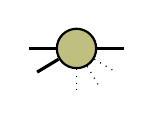
\begin{tikzpicture}[baseline=-0.5ex]
    \tikzset{tensor/.style = {minimum size = 0.5cm,shape = circle,thick,draw=black,inner sep = 0pt}, edge/.style = {thick,line width=.4mm},every loop/.style={}}
    \def\x{6}
    \node[tensor,fill=green!50!red!50!white] (T) at (\x,0) {$\Tt$};
    \draw[edge] (T) -- (\x-0.6,0);
    \draw[edge] (T) -- (\x+0.6,0);
    \draw[edge] (T) -- (\x-0.5,-0.3);
    \draw[dotted] (T) -- (\x,-0.6);
    \draw[dotted] (T) -- (\x+0.5,-0.3);
    \draw[dotted] (T) -- (\x+0.3,-0.5);
    \end{tikzpicture}.
$
我们用矩形、三角形、圆形等不同形状以及各种颜色来表示张量。形状与颜色主要起视觉提示的作用。
张量的\emph{阶}（order）指它的维度个数。例如，$N$ 阶张量 $\Tt\in\RR^{d_1\times\cdots\times d_N}$ 是由标量~$\Tt_{i_1,\dots,i_N}$ 构成的多维数组，由 $N$ 个指标 $i_1\in [d_1], i_2\in[d_2],\cdots, i_N \in [d_N]$ 索引。每个轴称为张量的一个\emph{模}（mode）：$N$ 阶张量有 $N$ 个模。
 
 张量把向量与矩阵自然推广为高维数组。阶数越高，这类数组的表示就越困难。\emph{张量网络}为表示和运算这些高阶对象提供了简单而直观的方式。借助张量网络的图示记法，可以更轻松地表达复杂的张量运算~\citep{biamonte2017tensor,orus2014practical}。


\paragraph{张量网络的节点}\label{def:tn-nodes}
在张量网络中，每个节点（node，或称顶点）表示一个张量，腿~（与之关联的边）的数目对应张量的阶：标量是没有边的节点，向量节点有一条边，矩阵节点有两条边，依此类推。例如，
\begin{center}
    
    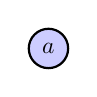
\begin{tikzpicture}[baseline=-0.5ex]
    \tikzset{tensor/.style = {minimum size = 0.5cm,shape = circle,thick,draw=black,inner sep = 0pt}, edge/.style = {thick,line width=.4mm},every loop/.style={}}
    \def\y{0}
    \def\x{0}
    \node[tensor,fill=blue!20!white] (a) at (\x,\y){\scalebox{0.85}{$a$}};
    \end{tikzpicture}%
    \ \ \ $\in \RR$,\hspace{0.01cm}
    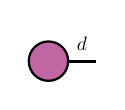
\begin{tikzpicture}[baseline=-0.5ex]
    \tikzset{tensor/.style = {minimum size = 0.5cm,shape = circle,thick,draw=black,inner sep = 0pt}, edge/.style = {thick,line width=.4mm},every loop/.style={}}
    \def\y{0}
    \def\x{0}
    \node[tensor,fill=blue!40!red!60!white] (a) at (\x,\y){\scalebox{0.85}{$\ab$}};
    \draw[edge] (\x+0.25,\y) -- (\x+0.6,\y)  node [midway,above] {\scalebox{0.7}{\dimcolor{$d$}}};
    \end{tikzpicture}
    $\in \RR^d$,\hspace{0.3cm}
    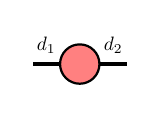
\begin{tikzpicture}[baseline=-0.5ex]
    \tikzset{tensor/.style = {minimum size = 0.5cm,shape = circle,thick,draw=black,inner sep = 0pt}, edge/.style = {thick,line width=.4mm},every loop/.style={}}
    \def\y{0}
    \def\x{0}
    \node[tensor,fill=red!50!white] (A) at (\x,\y){\scalebox{0.85}{$\Ab$}};
    \draw[edge] (\x+0.25,\y) -- (\x+0.6,\y)  node [midway,above] {\scalebox{0.7}{\dimcolor{$d_2$}}};
    \draw[edge] (\x-0.25,\y) -- (\x-0.6,\y)  node [midway,above] {\scalebox{0.7}{\dimcolor{$d_1$}}};
    \end{tikzpicture}
    \ \ \ $\in \RR^{d_1\times d_2}$,\hspace{0.3cm}
    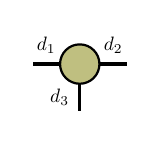
\begin{tikzpicture}[baseline=-0.5ex]
    \tikzset{tensor/.style = {minimum size = 0.5cm,shape = circle,thick,draw=black,inner sep = 0pt}, edge/.style = {thick,line width=.4mm},every loop/.style={}}
    \def\y{0}
    \def\x{0}
    \node[tensor,fill=green!50!red!50!white] (A) at (\x,\y){\scalebox{0.85}{$\At$}};
    \draw[edge] (\x+0.25,\y) -- (\x+0.6,\y)  node [midway,above] {\scalebox{0.7}{\dimcolor{$d_2$}}};
    \draw[edge] (\x-0.25,\y) -- (\x-0.6,\y)  node [midway,above] {\scalebox{0.7}{\dimcolor{$d_1$}}};
    \draw[edge] (\x,\y-0.25) -- (\x,\y-0.6)  node [midway,left] {\scalebox{0.7}{\dimcolor{$d_3$}}};
    \end{tikzpicture}
    \ \ \ $\in \RR^{d_1\times d_2\times d_3}$,\hspace{0.01cm}
    \begin{tikzpicture}[baseline=-0.5ex]
    \tikzset{tensor/.style = {minimum width = 1.8cm,minimum height = 0.4cm,shape = rounded rectangle,thick,draw=black,inner sep = 0pt}, edge/.style = {thick,line width=.4mm},every loop/.style={}}
    \def\x{0}
    \def\y{0}
    \draw[edge] (\x-0.2,\y-0.15) -- (\x-0.2,\y-0.6)node [midway,left=-0.05cm] {\scalebox{0.7}{\dimcolor{$d_2$}}};
    \draw[edge] (\x-0.6,\y-0.15) -- (\x-0.6,\y-0.6)node [midway,left=-0.05cm] {\scalebox{0.7}{\dimcolor{$d_1$}}};
    \draw[edge] (\x+0.2,\y-0.15) -- (\x+0.2,\y-0.6)node [midway,left=-0.05cm] {\scalebox{0.7}{\dimcolor{$d_3$}}};
    \draw[edge] (\x+0.6,\y-0.15) -- (\x+0.6,\y-0.6)node [midway,left=-0.05cm] {\scalebox{0.7}{\dimcolor{$d_4$}}};
    \node[tensor,fill=green!30!white] (Bt) at (\x,\y){$\Bt$};
    \end{tikzpicture}
    $\in \RR^{d_1\times d_2\times d_3\times d_4}$.

\end{center}
分别表示标量、向量、矩阵、三阶张量与四阶张量。
在本手册中，
\begin{itemize}
    \item 张量用带颜色的图形表示，称为节点，颜色与形状并无特定含义~（除非另有说明）。
    \item 标量用小写字母表示~（如 $a$），向量用粗小写字母表示~（如 $\vb$），矩阵用粗大写字母表示（如 $\Mb$），高阶张量则用
    粗花体大写字母表示~（如 $\Tt$）。
    \item 张量每个模的维数用一个灰色字母标在相应腿的上方，例如，
$
    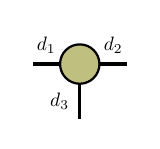
\begin{tikzpicture}[baseline=-0.5ex]
    \tikzset{tensor/.style = {minimum size = 0.5cm,shape = circle,thick,draw=black,inner sep = 0pt}, edge/.style = {thick,line width=.4mm},every loop/.style={}}
    \def\y{0}
    \def\x{0}
    \node[tensor,fill=green!50!red!50!white] (A) at (\x,\y){\scalebox{0.85}{$\At$}};
    \draw[edge] (\x+0.25,\y) -- (\x+0.6,\y)  node [midway,above] {\scalebox{0.7}{\dimcolor{$d_2$}}};
    \draw[edge] (\x-0.25,\y) -- (\x-0.6,\y)  node [midway,above] {\scalebox{0.7}{\dimcolor{$d_1$}}};
    \draw[edge] (\x,\y-0.25) -- (\x,\y-0.7)  node [midway,left] {\scalebox{0.7}{\dimcolor{$d_3$}}};
    \end{tikzpicture}
    \ \ \ \in \RR^{d_1\times d_2\times d_3},
$
是尺寸为 $d_1\times d_2\times d_3$ 的三阶张量。
    
$
\At_{i,j,k} = 
    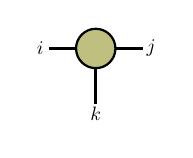
\begin{tikzpicture}[baseline=-0.5ex]
    \tikzset{tensor/.style = {minimum size = 0.5cm,shape = circle,thick,draw=black,inner sep = 0pt}, edge/.style = {thick,line width=.4mm},every loop/.style={}}
    \def\y{0}
    \def\x{0}
    \node[tensor,fill=green!50!red!50!white] (A) at (\x,\y){\scalebox{0.85}{$\At$}};
    \draw[edge] (\x+0.25,\y) -- (\x+0.6,\y)  node [pos=1.3] {\scalebox{0.7}{\indcolor{$j$}}};
    \draw[edge] (\x-0.25,\y) -- (\x-0.6,\y)  node [pos=1.3] {\scalebox{0.7}{\indcolor{$i$}}};
    \draw[edge] (\x,\y-0.25) -- (\x,\y-0.7)  node [pos=1.3] {\scalebox{0.7}{\indcolor{$k$}}};
    \end{tikzpicture}
$    
是三阶张量 $\At$ 的第 $(i,j,k)$ 个元素。
\end{itemize}
注意，大矩阵有时也可借助重排（reshaping）被视为高阶张量，例如，
\begin{align*}
    &\Tb
    =
    \begin{tikzpicture}[baseline=\baseline]
    \tikzset{tensor/.style = {minimum size = 0.5cm,shape = circle,thick,draw=black,inner sep = 0pt}, edge/.style = {thick,line width=.4mm},every loop/.style={}}
    \def\x{0}
    \def\y{0}
    \node[tensor,fill=green!50!blue!40!white] (Tb) at (\x,\y){$\Tb$};
    \draw[edge] (Tb) -- (\x+1.15,\y) node [midway,above] {\scalebox{0.7}{\dimcolor{$J_1J_2J_3J_4$}}};
    \draw[edge] (Tb) -- (\x-1.15,\y) node [midway,above] {\scalebox{0.7}{\dimcolor{$I_1I_2I_3I_4$}}};
    \end{tikzpicture}\in\RR^{I_1I_2I_3I_4\times J_1J_2J_3J_4}
    \equiv
    \Tt = 
    \begin{tikzpicture}[baseline=-0.5ex]
    \tikzset{tensor/.style = {minimum width = 1.8cm,minimum height = 0.4cm,shape = rounded rectangle,thick,draw=black,inner sep = 0pt}, edge/.style = {thick,line width=.4mm},every loop/.style={}}
    \def\x{0}
    \def\y{0}
    \draw[edge] (\x-0.2,\y-0.15) -- (\x-0.2,\y-0.6)node [midway,left=-0.05cm] {\scalebox{0.7}{\dimcolor{$I_2$}}};
    \draw[edge] (\x-0.6,\y-0.15) -- (\x-0.6,\y-0.6)node [midway,left=-0.05cm] {\scalebox{0.7}{\dimcolor{$I_1$}}};
    \draw[edge] (\x+0.2,\y-0.15) -- (\x+0.2,\y-0.6)node [midway,left=-0.05cm] {\scalebox{0.7}{\dimcolor{$I_3$}}};
    \draw[edge] (\x+0.6,\y-0.15) -- (\x+0.6,\y-0.6)node [midway,left=-0.05cm] {\scalebox{0.7}{\dimcolor{$I_4$}}};
    \draw[edge] (\x-0.2,\y+0.15) -- (\x-0.2,\y+0.6)node [midway,left=-0.05cm] {\scalebox{0.7}{\dimcolor{$J_2$}}};
    \draw[edge] (\x-0.6,\y+0.15) -- (\x-0.6,\y+0.6)node [midway,left=-0.05cm] {\scalebox{0.7}{\dimcolor{$J_1$}}};
    \draw[edge] (\x+0.2,\y+0.15) -- (\x+0.2,\y+0.6)node [midway,left=-0.05cm] {\scalebox{0.7}{\dimcolor{$J_3$}}};
    \draw[edge] (\x+0.6,\y+0.15) -- (\x+0.6,\y+0.6)node [midway,left=-0.05cm] {\scalebox{0.7}{\dimcolor{$J_4$}}};
    \node[tensor,fill=yellow] (Bt) at (\x,\y){$\Tt$};
    \end{tikzpicture}
    \in\RR^{I_1\times I_2\times I_3\times I_4\times J_1 \times J_2\times J_3\times J_4}.
\end{align*}
\paragraph{张量网络的边}\label{subsec:contraction} 在张量网络图中，腿分为两类：已收缩的腿~（连接两个张量的腿）与未收缩的腿，后者也称自由腿~（free legs），一端悬空~（即不与任何其他张量相连的腿）。如前所述，未收缩的腿对应自由指标（free index）：自由腿的数目给出张量的阶——标量没有自由腿，向量有一条，矩阵有两条，高阶张量则有三条或更多。已收缩的腿表示收缩（contraction）：
张量可沿尺寸相同的腿相连，这表示对所连接的模求和~（收缩）。
求和与收缩在本文中通用。最常见的收缩运算为\textit{矩阵乘法}。对两个矩阵 $\Ab\in\RR^{d_1\times R}, \Bb\in\RR^{R\times d_2}$，其矩阵乘积相当于 $\Ab$ 的第二模与 $\Bb$ 的第一模之间的收缩：

\begin{align}\label{eq:matrix-product}
(\Ab\Bb)_{ij} 
=
\begin{tikzpicture}[baseline=\baseline]
   \tikzset{tensor/.style = {minimum size = 0.5cm,shape = circle,thick,draw=black,inner sep = 0pt}, edge/.style = {thick,line width=.4mm},every loop/.style={}}
    \def\y{0}
    \def\x{0}
    \node[tensor,fill=red!50!white] (A) at (\x,\y){\scalebox{0.85}{$\Ab$}};
    \node[tensor,fill=blue!50!white] (B) at (\x+1,\y){\scalebox{0.85}{$\Bb$}};
    \draw[edge] (A) -- (B) node [above,midway] {\scalebox{0.7}{\dimcolor{$R$}}};
    \draw[edge] (\x-0.25,\y) -- (\x-0.75,\y)  node [pos=1.3] {\scalebox{0.7} {\indcolor{$i$}}};
    \draw[edge] (\x+1.25,\y) -- (\x+1.75,\y)  node [pos=1.3] {\scalebox{0.7}{\indcolor{$j$}}};
    \end{tikzpicture}
= \sum_{r=1}^R\Ab_{ir}\Bb_{rj},\ \ \ \text{for}\ \ i\in[d_1],j\in[d_2]\ .
\end{align}
由于该等式对一切指标 $i$ 与 $j$ 都成立，可以直接简写为
\begin{align}\label{eq:matrix-product_noidx}
\Ab\Bb 
=
\begin{tikzpicture}[baseline=\baseline]
   \tikzset{tensor/.style = {minimum size = 0.5cm,shape = circle,thick,draw=black,inner sep = 0pt}, edge/.style = {thick,line width=.4mm},every loop/.style={}}
    \def\y{0}
    \def\x{0}
    \node[tensor,fill=red!50!white] (A) at (\x,\y){\scalebox{0.85}{$\Ab$}};
    \node[tensor,fill=blue!50!white] (B) at (\x+1,\y){\scalebox{0.85}{$\Bb$}};
    \draw[edge] (A) -- (B) node [above,midway] {\scalebox{0.7}{\dimcolor{$R$}}};
    \draw[edge] (\x-0.25,\y) -- (\x-0.75,\y)  node [midway, above] {\scalebox{0.7}{\dimcolor{$d_1$}}};
    \draw[edge] (\x+1.25,\y) -- (\x+1.75,\y)  node [midway,above] {\scalebox{0.7}{\dimcolor{$d_2$}}};
    \end{tikzpicture}
 \ \in \mathbb R^{d_1\times d_2}.
\end{align}

